\documentclass[11pt,a4paper]{article}
\usepackage[T1]{fontenc}
\usepackage[utf8]{inputenc}
\usepackage[margin=22mm]{geometry}
\usepackage{amsmath,booktabs,graphicx,hyperref}
\title{Assessment of Rogelio Palomo's v2 CSA}
\author{NAUSICA calculation record}\date{\today}
\begin{document}\maketitle
The v2 circuit reduces output noise but also reduces the voltage produced by
an arriving ion. Under the paper's input and readout conditions, its
input-equivalent noise is 179.1 electrons RMS, compared with 112.7 for
the circuit currently used in the paper. The calculation retains the supplied
v2 transistor dimensions and gate voltages.

\section*{Circuits and conditions}
The v2 M4 has $W=0.54\,\mu$m, $L=2.4\,\mu$m and gate voltage 0.64 V.
Its M3 has $W=50\,\mu$m, $L=0.5\,\mu$m and gate voltage 0.6 V.
The paper circuit uses M4 with $W=2.88\,\mu$m, $L=1.44\,\mu$m and
gate voltage 0.556803 V; M3 has $W=200\,\mu$m, $L=2\,\mu$m and gate
voltage 0.538477 V. All cases use a 3 fF feedback capacitor and 1.8 V supply.

The native v2 conditions are 0.25 pF external input capacitance and
$27\,^{\circ}$C. The matched comparison uses 1.25 pF and $20\,^{\circ}$C
for both circuits. A third calculation combines the v2 M4 and its gate bias
with the paper's enlarged M3 and its adjusted gate bias.

\section*{Reproduction and model syntax}
LTspice 17.2.4 for macOS reproduces the supplied Windows 26.0.1 spectrum
over 1 Hz--1 GHz with maximum relative difference $7.6e-08$, using the
supplied model card unchanged. The card contains \texttt{NOIBE} where
\texttt{NOIB} is intended. The supplied log reports an unknown parameter.
The corrected calculation replaces this spelling and closes the model
parentheses, using the same corrected card as the paper. At 1 Hz the output
noise amplitude density changes from 214.35 to 215.66
$\mu$V/$\sqrt{\mathrm{Hz}}$.

\section*{Operating point and voltage gain}
\begin{center}\begin{tabular}{lrrr}\toprule
Circuit & Baseline (V) & $|V_{\rm out}/V_{\rm in}|$ at 1 Hz & M4 $1/g_{ds}$ (M$\Omega$)\\\midrule
Paper circuit & 0.879 & 816.6 & 28.8 \\
v2, native conditions & 1.663 & 13.4 & 66.7 \\
v2, matched conditions & 1.646 & 16.8 & 59.9 \\
v2, retuned gate & 0.879 & 941.7 & 50.3 \\
\bottomrule\end{tabular}\end{center}
The voltage ratio is measured by an AC current excitation with the feedback
network connected, preserving the operating point. The resistance is M4's
intrinsic small-signal drain resistance, read from the operating-point log
at its printed precision. It is distinct from the output resistance of the
complete amplifier. The matched v2 output lies near the positive supply;
M5 has only 30.6 $\mu$V between drain and source. The increased M4
resistance therefore accompanies a much lower amplifier voltage gain at
the supplied bias.

Changing only the v2 M4 gate voltage to 0.651398349 V restores an output
baseline of 0.878932 V. The transistor dimensions, M3 and other biases
are unchanged. The per-ion gain then rises to 29.095 $\mu$V/ion,
demonstrating that the small signal at the supplied bias comes from the
operating point. The ENC is 179.7 electrons RMS: output noise rises
along with signal gain. This variant is a separate bias-adjustment study.

\section*{Ion current, readout and sensitivity}
The current is that of a central square pad of 0.5 mm side in an infinite
grounded plane, with homogeneous gas in the upper half-space. The weighting
potential is one on the pad, zero on the surrounding plane, and zero at
infinity. Ions approach centrally at 3 m/s through the final 5 mm, with mean
collection times uniformly distributed over 20 ms. Each ion contributes
$e\,\Delta\phi_w$ on this finite path. The input waveform is reused from the
saved Julia calculation without renormalization or an extra collection pulse.

The voltage is averaged over centred 300 $\mu$s windows at consecutive frame
boundaries. The measured signal is
$D=-(\overline V_1-\alpha\overline V_0)$, where
$\alpha=\exp(-20\,\mathrm{ms}/\tau)$.
Each circuit's $\tau$ is obtained from its 100-ion, current-free tail over
21--120 ms. Noise uses the quiescent SPICE one-sided output spectrum over
0.1 Hz--1 MHz, filtered by the same averaging and frame difference.
The one-ion gain $g$ defines $\mathrm{ENC}=\sigma_D/g$. The final column
is checked using finite-count transients on both sides of $S/N=5$.

\begin{center}\begin{tabular}{lrrrr}\toprule
Circuit & $g$ ($\mu$V/ion) & $\sigma_D$ (mV) & ENC ($e$ RMS) & Minimum ions\\\midrule
Paper circuit & 27.119 & 3.056 & 112.7 & 564 \\
v2, native conditions & 1.547 & 0.185 & 119.9 & 597 \\
v2, matched conditions & 1.129 & 0.202 & 179.1 & 890 \\
v2 with enlarged M3 & 1.170 & 0.166 & 142.0 & 707 \\
v2, retuned gate & 29.095 & 5.228 & 179.7 & 900 \\
\bottomrule\end{tabular}\end{center}

\begin{figure}[htbp]\centering
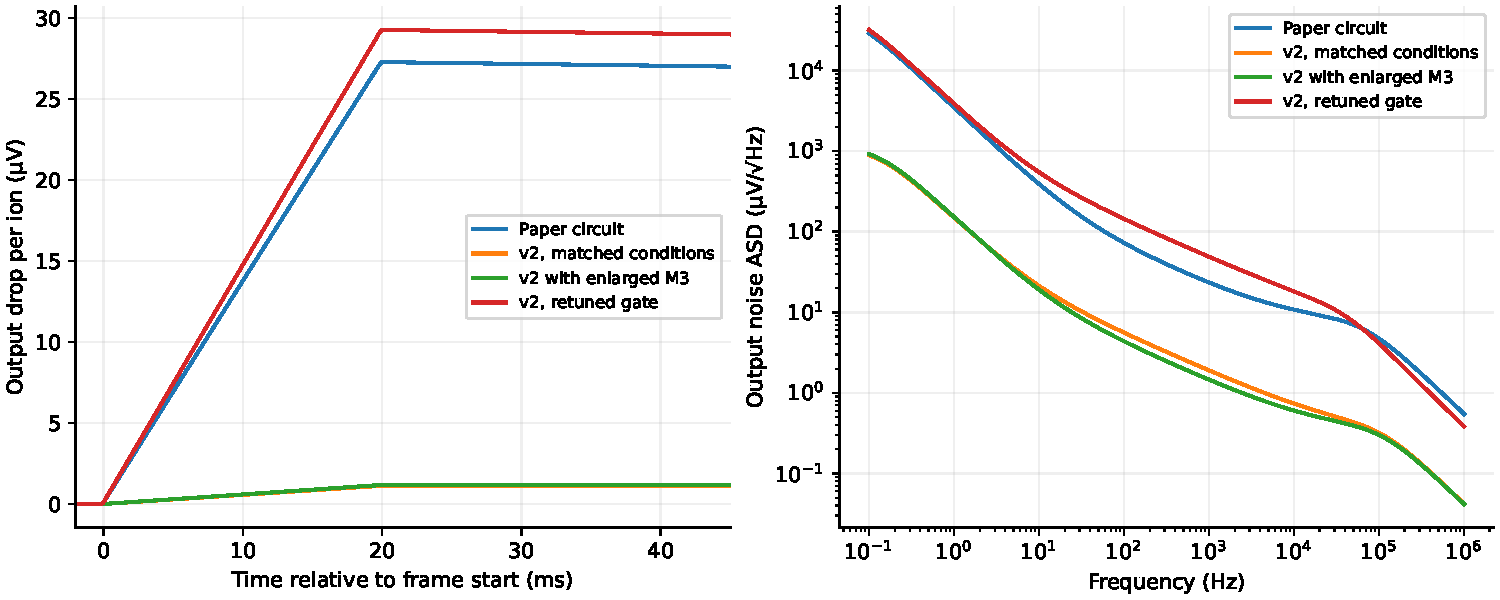
\includegraphics[width=\linewidth]{response_noise.pdf}
\caption{Matched input capacitance and temperature. Left: voltage response
to the uniform-arrival current, normalized per ion. Right: quiescent output
noise spectrum.}
\end{figure}

\section*{Numerical checks}
Both 5 and 2.5 $\mu$s maximum time steps are evaluated, with transient
tolerances tightened from $(10^{-5},10^{-17}\,\mathrm A,10^{-8}\,\mathrm V)$
to $(5\times10^{-6},5\times10^{-18}\,\mathrm A,5\times10^{-9}\,\mathrm V)$
for relative, current and voltage tolerances. The more stringent inherited
voltage tolerance of $10^{-10}$ V caused the v2 zero-input transient to stall
in this simulator. The table gives the successful paired-refinement errors.
Frequency densities of 200 and 400 points per decade and independent
Gauss quadrature orders of 8 and 16 check the noise integral. Charge
conservation is checked against the finite-path input charge.

\begin{center}\small\begin{tabular}{lrrrr}\toprule
Circuit & $\tau$ (s) & Signal error & Noise error & Fit residual\\\midrule
v2, native conditions & 0.6822 & 7.3e-06 & 7e-07 & 1.4e-06 \\
v2, matched conditions & 1.2300 & 7.8e-06 & 5.6e-07 & 3.4e-07 \\
v2 with enlarged M3 & 1.2395 & 1.2e-05 & 7.1e-07 & 3.7e-07 \\
\bottomrule\end{tabular}\end{center}
The gain is also checked for 10, 100, 564, 1000 and 2000 ions, and for the
counts that bracket the threshold. In the matched v2 case its largest change
relative to the one-ion gain is 1.44\% over the tested range.
This weak nonlinearity is included in the threshold calculation.

\section*{Reproduction}
Configuration: \texttt{config/rogelio\_v2.toml}. Acquisition:
\texttt{scripts/run\_rogelio\_v2.py}. Julia analysis:
\texttt{src/ion\_signal/rogelio\_v2.jl}. Presentation:
\texttt{scripts/present\_rogelio\_v2.py}.
The pipeline command and full data locations are in
\texttt{results/ltspice/rogelio\_v2/README.md}. Supplied files and the
paper's historical results are preserved. This report is generated from HDF5.
\end{document}
